\documentclass[conference]{IEEEtran}
\usepackage[USenglish]{babel}
\usepackage{graphicx}
\usepackage{cite}
\usepackage{amsmath}
\usepackage{graphicx}
\usepackage{graphics}
\usepackage{psfrag}
\usepackage{pstricks}
\usepackage{color}
\usepackage{amsmath}
\usepackage{rotating}
\usepackage{setspace}
\usepackage{cite} % ordena as citacoes
\usepackage[T1]{fontenc}
\usepackage{mathtools, cuted}
\usepackage{subfig}
\usepackage{caption}
%\usepackage{subfigure}
%\usepackage[export]{adjustbox}

%\ifCLASSINFOpdf
%\else
% * <jose.avalos@utec.edu.pe> 2017-07-01T20:45:07.865Z:
%
% ^.
%\fi
%\hyphenation{op-tical net-works semi-conduc-tor}

\newcommand{\x}{\mathbf x}
\newcommand{\q}{\mathbf q}
\newcommand{\f}{\mathbf f}
\newcommand{\e}{\mathbf e}


\begin{document}
%%%%%%%%%%%%%%%%%%%%% TITLE %%%%%%%%%%%%%%%%%%%%%%%%%%%%%%%%%%
%\title{Image-driven robot-based drawing system itation of Human Drawing by a NAO Robot}
\title{Control of a mobile robot based on Potential field and Polar control}
\author{\IEEEauthorblockN{Jose-Maria Munoz, Emanuel S. Munoz, Oscar E. Ramos}
\IEEEauthorblockA{Department of Electrical Engineering, Universidad de Ingenieria y Tecnologia - UTEC, Lima, Peru}
}
% \author{\IEEEauthorblockN{Jose-Maria Munoz\IEEEauthorrefmark{1}, Jose Avalos\IEEEauthorrefmark{1}
% Oscar E. Ramos\IEEEauthorrefmark{1}}
% \IEEEauthorblockA{\IEEEauthorrefmark{1}Department of Electrical Engineering, Universidad de Ingenieria y Tecnologia - UTEC, Lima, Peru.}
% }
\maketitle
\begin{abstract}

\end{abstract}
\IEEEpeerreviewmaketitle
% \textbf{\textit{Keywords - NAO Robot, Inverse Kinematics, Image Processing, Drawing Imitation}}

\section{Introduction}

Mobile robots have become an extended field of research due to its applications in exploration and navigation on ground, see for example \cite{Desouza}\cite{Bonin-Font2008}. In practice, the differential wheeled robot is widely used because its dynamics and physical structure are not complex. However, the application in navigation of these robots deals with some problems for the controllability of its kinematics.

The robot is a non-holonomic system, so the controllability of these robots is difficult to achieve. This issue is currently presented when is needed a trajectory tracking in a closed environment. For example, the robot can not achieve a goal smoothly because its orientation is significantly important to its motion. The treatment of this problem has gone through different approaches, see \cite{Rubayat}\cite{Samson}\cite{Sung-On}. In general, the approaches can be divided for the model in a different system of coordinates. The recent research has dealt with it using polar coordinates, because it eliminates some constraints given in the Cartesian coordinate system. According to \cite{Matoui}, the control laws based on these coordinates have the potential to achieve an exponential stability smoothly through a closed-loop control. However, the mathematical formulation of these control laws do not consider trajectory constraints. The polar control laws can be used for obstacle avoidance if it is stated middle goals in which the robot can avoid them. However, these middle goals must be formulated arbitrarily, which is not a good approach for the autonomy of the robot in a navigation task.

On the other hand, the practical application of these robots deals with an environment with obstacles, so it is necessary to overcome this limitation of the control.  One of the most common methods to solve the path planning problem is artificial potential field (APF). The research in this field has shown that APF is an immediate alternative on mobile robots, see \cite{Woods}\cite{Merheb}. However, for the two-wheeled robot, its non-holonomic problem impede a normal path planning through this method. The artificial attractive or repulsive forces formulate trajectories which the robot cannot follow through conventional control methods. 

In this work, the authors propose a control based on potential field and on polar control laws for the kinematics of the two-wheeled robot, so it can achieve smoothly a validated trajectory to reach to a position goal. Experimental results were obtained through the implementation of each individual controller in a Kobuki model for a virtual workspace in Gazebo simulator. Posteriorly, the integration of the controllers for obtaining the proposed control is implemented in a real Kobuki robot powered with a Lidar sensor for obtainment of position obstacles. 
 
This work is structured as follows. In section "", it is introduced the forward and inverse kinematics. Section "" formulates the potential field equation for its application as well as it is stated the control laws in the polar coordinate system. The section "" it presents the control system integration and its implementation in the Kobuki robot through the ROS system. Finally, the experimental results and conclusion are shown to give details of the implementation.

\section{Robot Motion Generation}
\label{sec:robot_motion}
For a navigation approach in a wheeled differential robot, it is necessary to control its motion appropriately. In this section, it is shown the kinematics of the robot and the control laws for its motion.

\subsection{Polar controller}

\begin{figure}[h]
  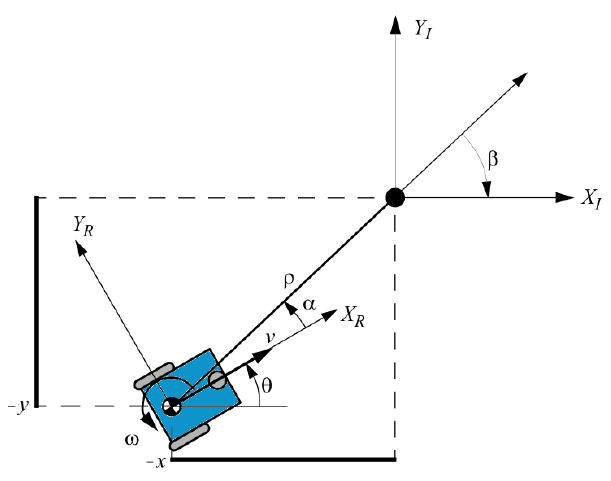
\includegraphics[width=0.5\linewidth]{control_polar.png}
  \centering\caption{Feedback control of states to a reference position}
  \label{fig:Polar}
\end{figure}

An alternative way of getting a soft control about position and orientation for a differential robot is throughout a control linear law for feedback  of the states based on polar coordinates.Without lost of generality a $\textbf{$X_{I}$,$Y_{I}$}$ reference system is associated to the position and orientation desired with orientation  set for the orientation desired.The diagram shows that on Figure ~\ref{fig:Polar} where $\textbf{$X_{R}$,$Y_{R}$}$ represent the reference system of the proper robot.

The angle $\theta$ represents the robot orientation and the angles $\alpha$ and $\beta$ are defined as they are shown in the figure \ref{fig:Polar}. The robot position is ($x_{d}$-$x$, $y_{d}$-$y$) in the inertial reference system. And the distance until the desired point is represented by $\rho$. When $\alpha \leq \pi/2 $ is set up, the desired point is located in front of the robot and you have:
\begin{equation}
	\rho = \sqrt[]{(x_{d} - x)^2 + (y_{d} - y)^2} 
\end{equation}
\begin{equation}
	\alpha = atan2(y_{d} - y, x_{d} - x) - \theta 
\end{equation}
\begin{equation}
	\beta = -atan2(y_{d} - y, x_{d} - x) + \theta_{d}.
\end{equation}

Considering these variables shown, the following control law can be used for the linear speed and for the angular velocity of the robot:

\begin{equation}
	v = k_{\rho}\rho
\end{equation}
\begin{equation}
	\omega = k_{\alpha}\alpha + k_{\beta}\beta
\end{equation}


\section{Path Generation}
\label{sec:APF}
\subsection{Artificial Potential Field}
There are several approaches in path planning through potential field. In this case, we opted for a one which considers some assumptions for its implementation. Given the potential field generates a force field, it is posteriorly used a guide to generate middle-goals for the polar control. In that way, it is only necessary the positions of the robot, the goal and the obstacles, so it could be generated a vector field from the sum of the attractive  and repulsive potential field.\\

\subsubsection{\textbf{Attractive Potential Field}}
The attractive potential field drives the robot to the goal position respect to the distance between them. Lets define a scalar potential field which depends on the distance between the current position of the robot $q$ and the goal position $q_{goal}$ as follows. 
\begin{equation}
	U_{att}(q) = \frac{1}{2} \zeta d^2(q,q_{goal})
	\label{eq:pot_attr}
\end{equation}

where  $\zeta$  is a parameter used to scale the effect of the attractive potential. The gradient of this field provides a vectorial field which points always to the desired goal position.

\begin{equation}
	\label{gradient_att}
	\begin{aligned}
		\nabla U_{att}(q) &= \nabla (\frac{1}{2}\zeta d^2 (q,q_{goal})),\\
		&=\frac{1}{2}\zeta \nabla d^2(q,q_{goal})\\
		&= \zeta(q - q_{goal})
	\end{aligned}
\end{equation}

The gradient vector points away from the goal with magnitude $\zeta$ at all points of the configuration space except the goal, where it is undefined. Starting from any point other than the goal, by following the negated gradient, a path is traced toward the goal. The equation \ref{gradient_att} is a vector based at $q$, points away from $q_{goal}$, and has a magnitude proportional to the distance from $q$ to $q_{goal}$.\\

\subsubsection{\textbf{Repulsive Potential Field}}

A repulsive potential keeps the robot away from an obstacle. The strength of the repulsive force depends upon the robot's proximity to the obstacle. The closer the robot is to an obstacle, the stronger the repulsive force should be. Therefore, the repulsive potential is usually defined in terms of distance to the closest obstacle $D(q)$.

\begin{equation}
	U_{rep}(q) = 
		\begin{cases}
			\frac{1}{2}\eta(\frac{1}{D(q)} - \frac{1}{Q*})^2, & D(q)\leq Q*, \\
			0, & D(q) > Q*,
		\end{cases}
	\label{eq:pot_rep}
\end{equation}

whose gradient is
\begin{equation}
	\nabla U_{rep}(q) = 
		\begin{cases}
			\eta (\frac{1}{Q*} - \frac{1}{D(q)})\frac{1}{D(q)^2} \nabla D(q), &D(q) \leq Q*,\\
			0 , &D(q) > Q*,
		\end{cases}
	\label{eq:force_rep}
\end{equation}

where the $Q* \in R $ factor allows the robot to ignore obstacles sufficiently far away from it and the $\eta$ can be viewed as a gain on the repulsive gradient. These scalars are usually determined by trial and error.


\section{Results}
The proposed methodology was tested on a real Kobuki mobile robot. ROS was used to program the mobile robot. This section is divided into two subsections which are:

\subsection{Artificial Potential Field}

Potential field was implemented so that you can perform different tasks in different situations and thus have a robust behavior. This algorithm works with forces of atrraccion and repulsion. The first is used to reach the desired position and the second force is to avoid obstacles. These forces were decomposed in magnitude and direction so that the robot can take semi desired positions for each iteration.
To check the efficiency of the algorithm, it was simulated graphically in a workspace where the vector field was projected, indicating the potential field algorithm forces for different positions of the obstacles and the desired position.The forces of atrraccion can be observed in Figure \ref{f:apf}(a), where the desired position is $ (10,4) $ and the initial position of the robot is $ (2,18) $. The white points within the image refer to the desired semi-positions forming the path of the robot. You can also see that all the arrows in the vector field are in the direction of the robot's goal. Likewise, also in Figure \ref{f:apf}(b) you can see three obstacles that are distributed in different positions of the workspace. Each obstacle is projected as a red circle due to its high magnitude within its potential field, where the forces point outward in each obstacle. Finally, for the force of navigation, the forces of attraction and repulsion had to be superimposed, as shown in Figure \ref{f:apf}(c). Where the white points is the trajectory that the robot would generate assuming that this robot has a controller that overcomes non-holonomicity without having restrictions for its movement.

%Potential field fue implementado para que pueda realizar diferentes tareas en diversas situaciones y así tener un comportamiento robusto. Este algoritmo trabaja con fuerzas de atrraccion y repulsion. El primero es utilizado para llegar a la posicion deseada y la segunda fuerza es para evitar obstaculos. Estas fuerzas fueron descompuestas en magnitud y direccion para que el robot pueda tomar semi posiciones deseadas para cada iteracion.
%Para comprobar la eficiencia del algoritmo se simulo de forma gráfica en un espacio de trabajo donde se proyectó el campo vectorial indicando las fuerzas del algoritmo potential field para diferentes posiciones de los obstaculos y de la posicion deseada. 
%Las fuerzas de atrraccion se pueden observar en la Figura \ref{f:apf}(a), donde la posición deseada es $(10,4)$ y la posicion inicial del robot es $(2,18)$. Los puntos de color blanco dentro de la imagen hacen referencia a las semi posiciones deseadas formando la trayectoria del robot. Tambien se puede ver que todas las flechas,del campo vectorial,estan en direccion hacia la meta del robot. Asimismo, también en la Figura \ref{f:apf}(b) se puede observar a tres obstaculos que estan distribuidos en diferentes posiciones del espacio de trabajo. Cada obstaculo se proyecta como un circulo rojo debido a su alta magnitud dentro de su campo potencial, donde las fuerzas apuntan hacia afuera en cada obstaculo. Finalmente, para la fuerza de navegacion se tuvo que superponer las fuerzas de atraccion y repulsion como se observa en la Figura \ref{f:apf}(c). Donde los puntos blancos es la trayectoria que generaría el robot asumiendo que este robot tiene un controlador que supera la no holonomicidad no teniendo restricciones para su movimiento.

\begin{figure}[ht!]
	\centering
	\subfloat[Attractive Force]{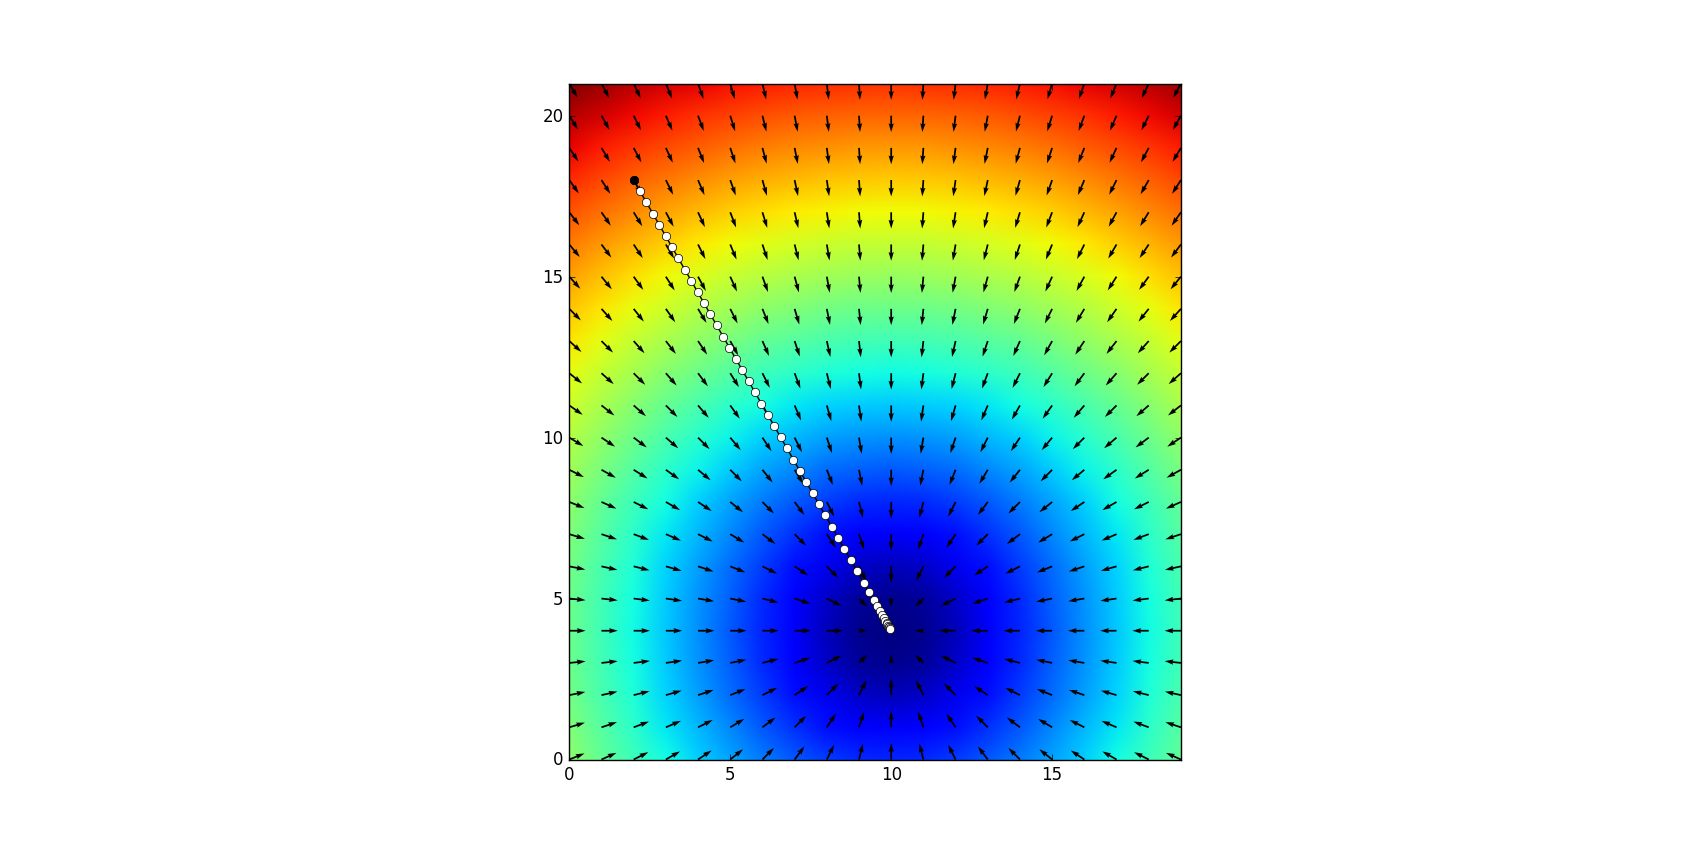
\includegraphics[width=40mm]{attr_force.png}}
	~\subfloat[Repulsive Force]{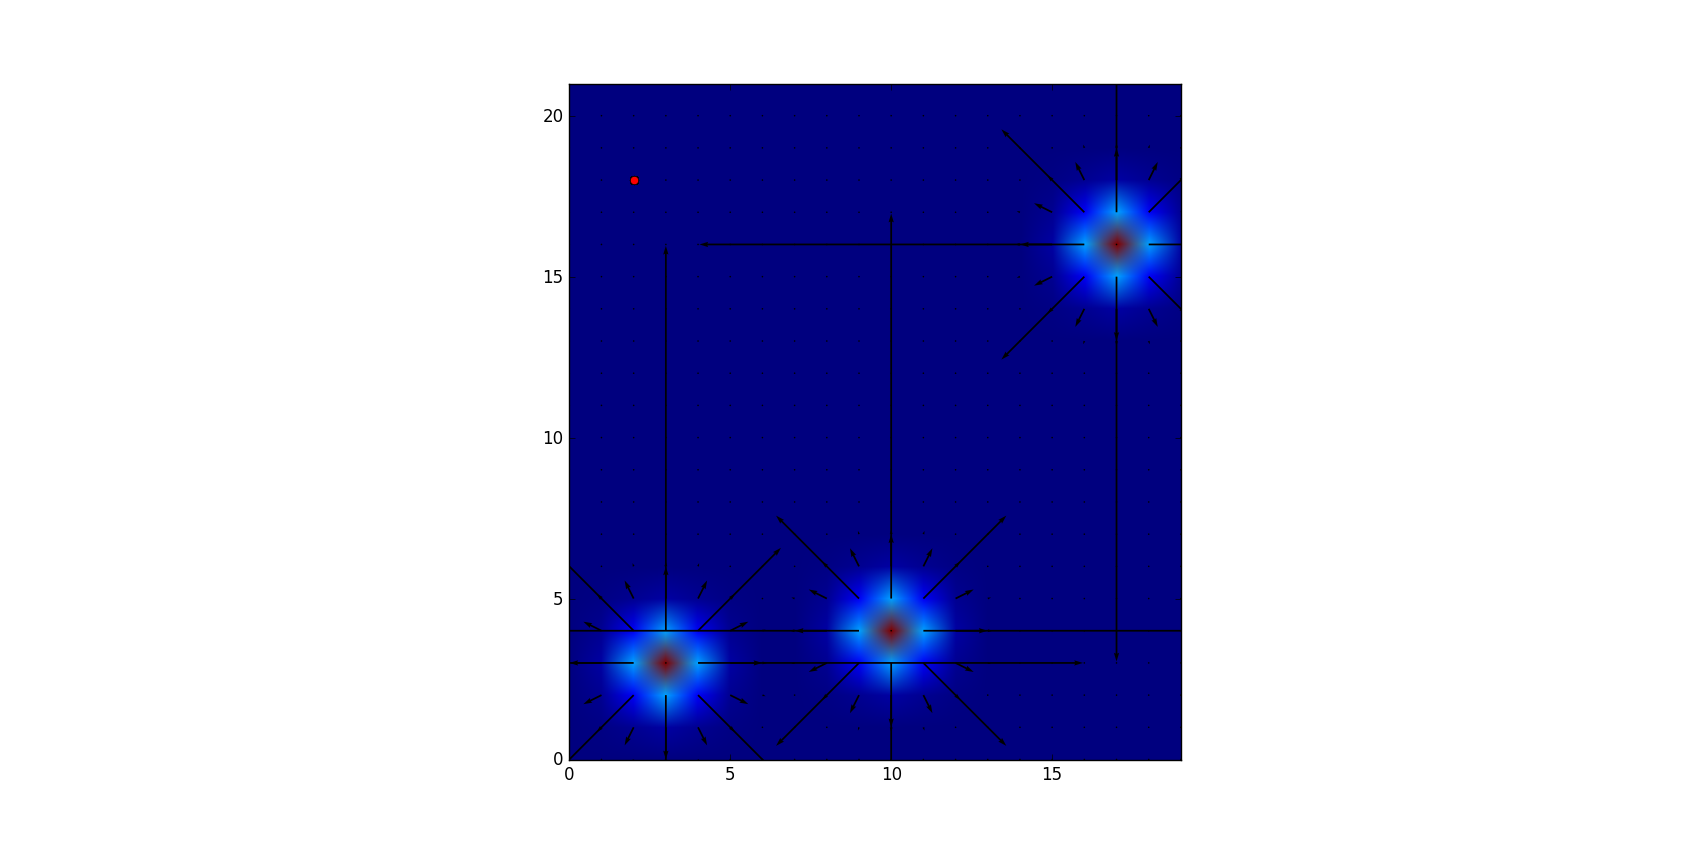
\includegraphics[width =40mm]{rep_force.png}}\\
	\subfloat[Navigation Force]{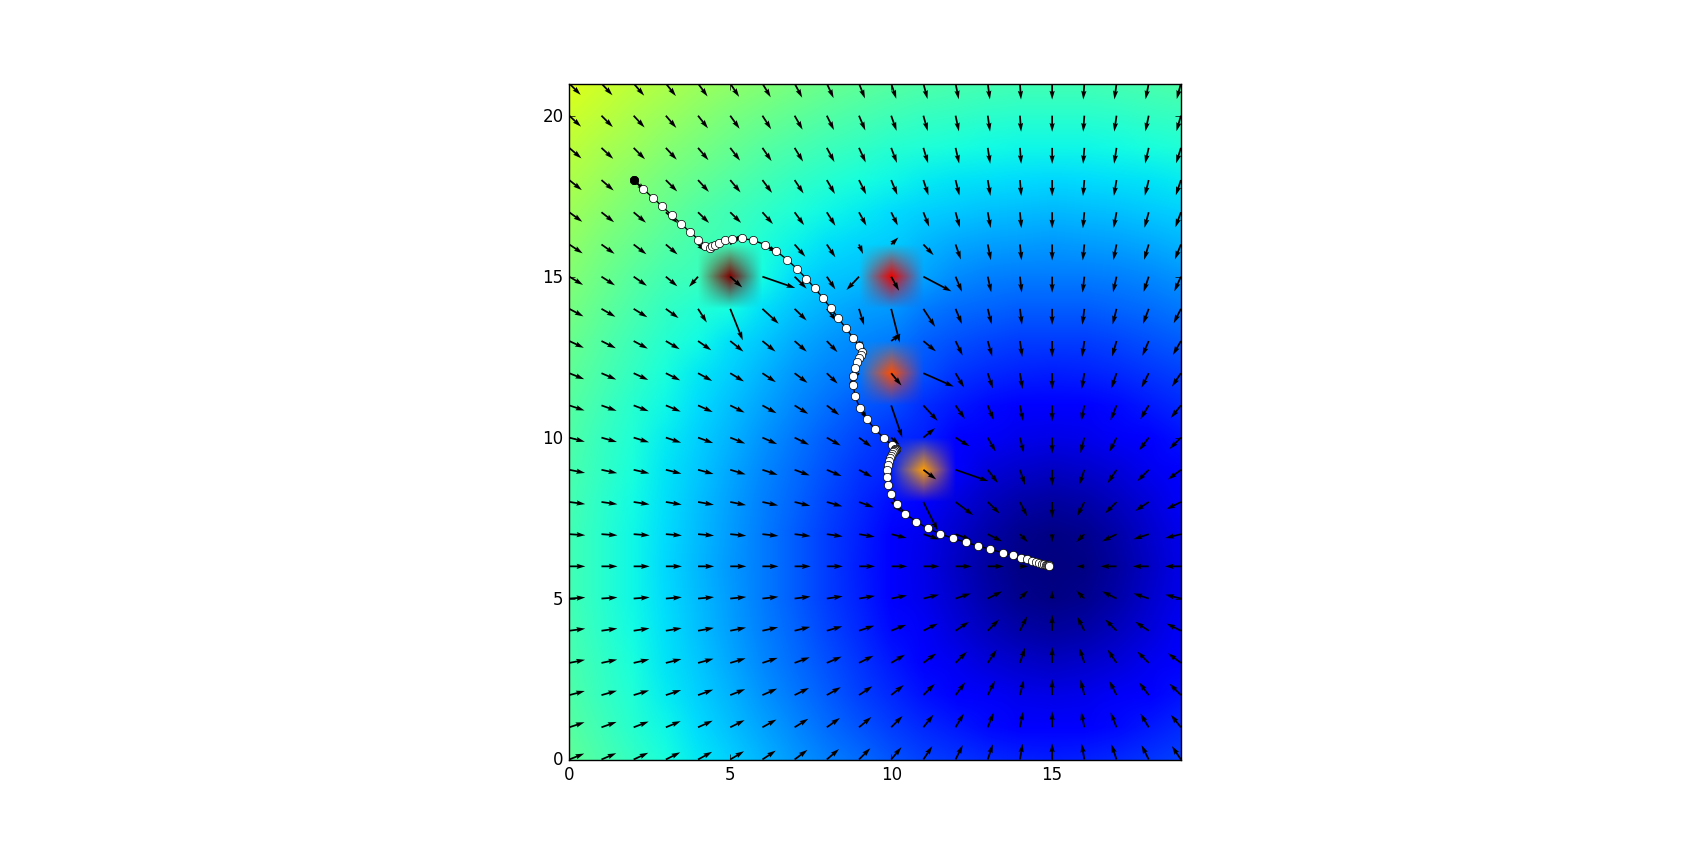
\includegraphics[width =40mm]{nav_force.png}}
%\subfloat[Attractive Force]{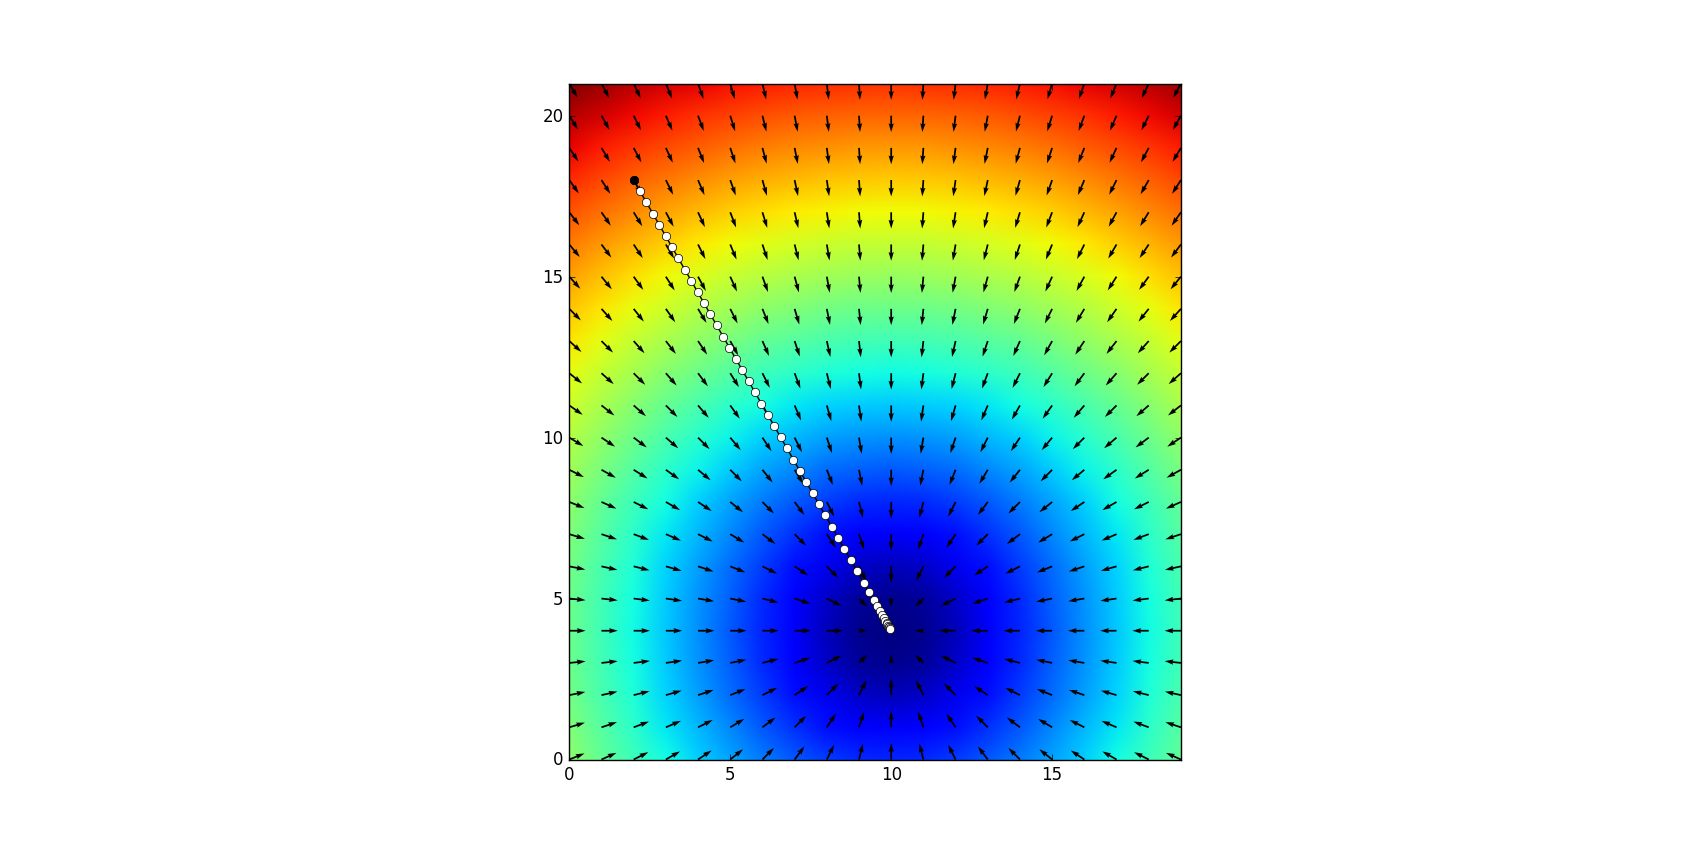
\includegraphics[width = 150mm]{attr_force.png}}
	\caption{Potential Field Algorithm} \label{f:apf}
\end{figure}

\subsection{Polar controller}

The polar controller was implemented for the Kobuki motion in a virtual workspace in Gazebo with no obstacles. The prompt of the proofs was the robot to achieve a given a random goal position.  It was considered a start position in the origin of the frame and the desired position ($x,y,\theta$) respect to the same inertial frame. The state variables (velocity, position and orientation) of the robot was obtained from odometry. The performance of the robot for one of the experimental cases is shown in the following figures.

The graphical results show the performance of the robot for a goal position () and orientation (). The start time of simulation is approximately 7 seconds because of a delay of the software. For every figure, the variation of the variable is immediate and in a homogeneous convergence time. In contrast, the figure []  shows a rapid convergence of the position compared to the other variables. In the same way, in figure [], there is a peak in the curve which diverges from the goal orientation. These results proves an over-dependence of the controller to the position instead of the orientation. This characteristic is mainly upward for a navigation resolution.

\begin{figure}
	\centering
	\subfloat[time vs position]{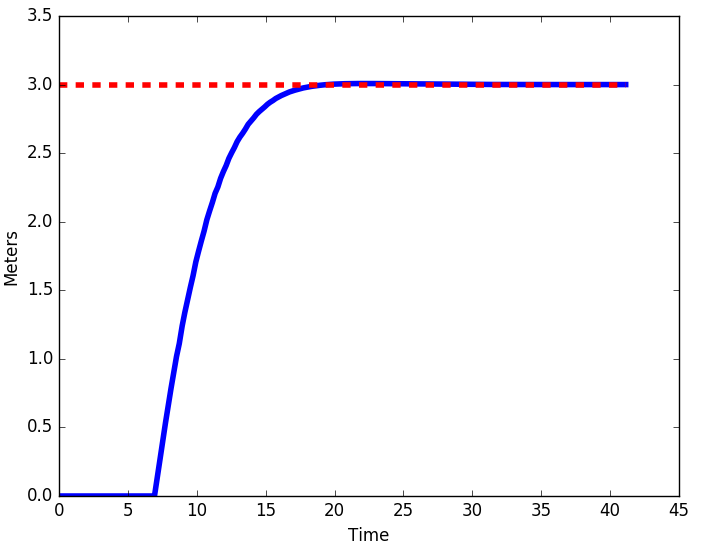
\includegraphics[width = 40mm]{tvsxy_tesis.png}}
	~\subfloat[time vs linear velocity]{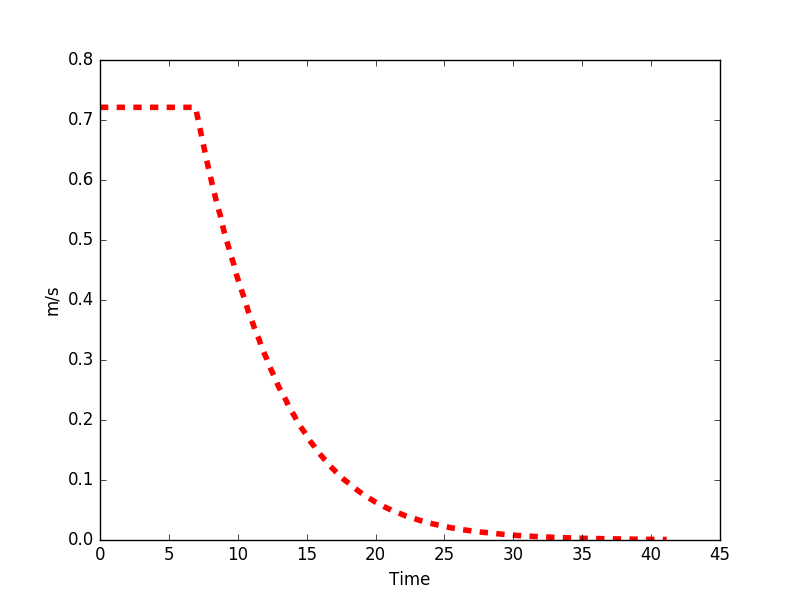
\includegraphics[width = 40mm]{tvsv_tesis.png}}\\
	\subfloat[time vs theta]{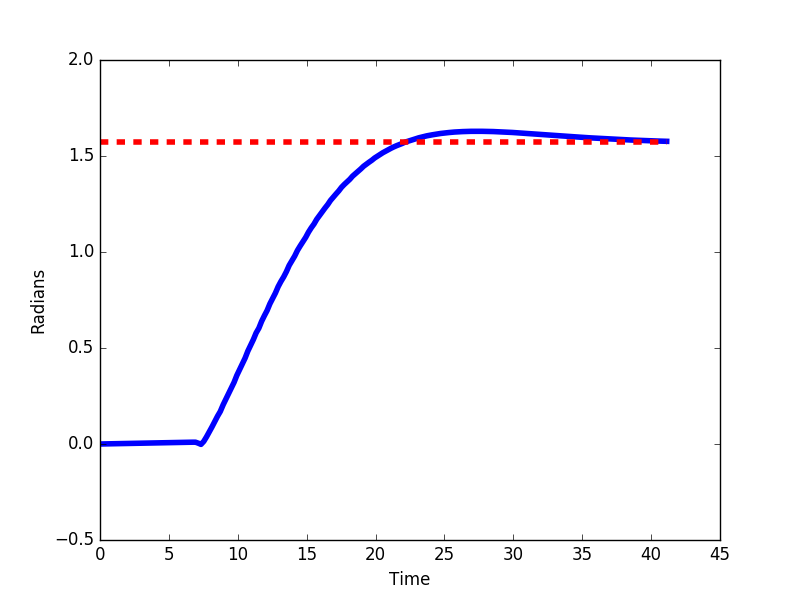
\includegraphics[width = 40mm]{tvstheta_tesis.png}}
	~\subfloat[time vs angular velocity]{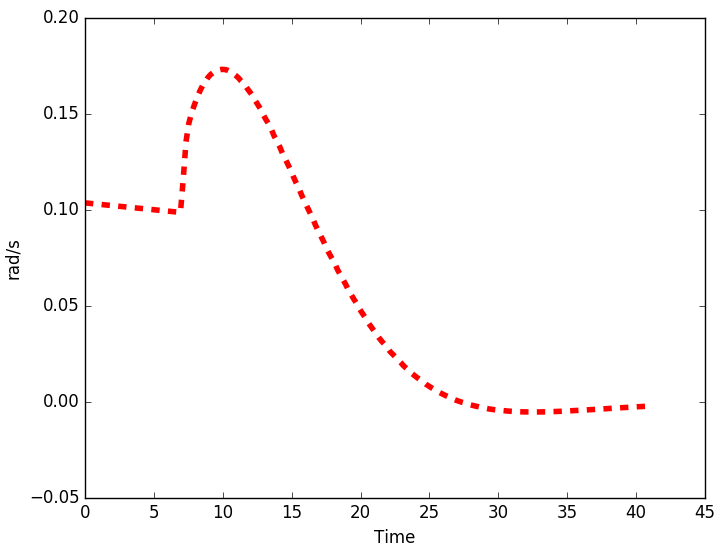
\includegraphics[width = 40mm]{tvsomega_tesis.png}}
	\caption{Polar controller for desired position $x=3, y=3, \theta=90°$} \label{f:polar}
\end{figure}

\subsection{Autonomous Navigation}
The proposed controller was implemented through an iterative algorithm for the Kobuki robot in a fixed environment. The algorithm takes middle goal position iteratively through the artificial potential field and it is drived by the polar controller to achieve them. We exposed to the robot to different obstacles whose positions were stated from a measurement of the physical of the environment, so it was not sensed by the robot. The performance of the robot is  shown in the following figures:

Figure \ref{f:kbki}(a) is composed of the attractive forces for every position(red dots) in which the algorithm is iterated in the two-dimensional environment within robot motion. It proves that for every position the attractive potential field drives the robot to the goal position. The trajectory shown in this figure is not forward to the goal because of the obstacles, which are not considered for the attractive APF. 

Figure \ref{f:kbki}(b) is composed for the repulsive forces for every iteration in the same 2D environment. The obstacles are shown in the graphic as green markers. The forces are only applied, as it was formulated above, for less than a arbitrarily range (for this result it was considered 1 meter). For each obstacle, the magnitude of the forces  increases as long as the robot is closer to it. Also, its direction points toward to the position of the robot, so it bring an opposite force to the attractive potential field.

Figure \ref{f:kbki}(c) shows the superposition of the forces with the actual obstacles. Each forces provides a middle goal position for the robot, thus it is the input variable for the polar controller. Even though the forces close to the obstacles have a high rate of change, the trajectory is smooth. It demonstrates the effectiveness of the polar controller despite its non-holonomic charateristic. 
\begin{figure}
	\centering
	\subfloat[Attractive force applied to the mobile robot]{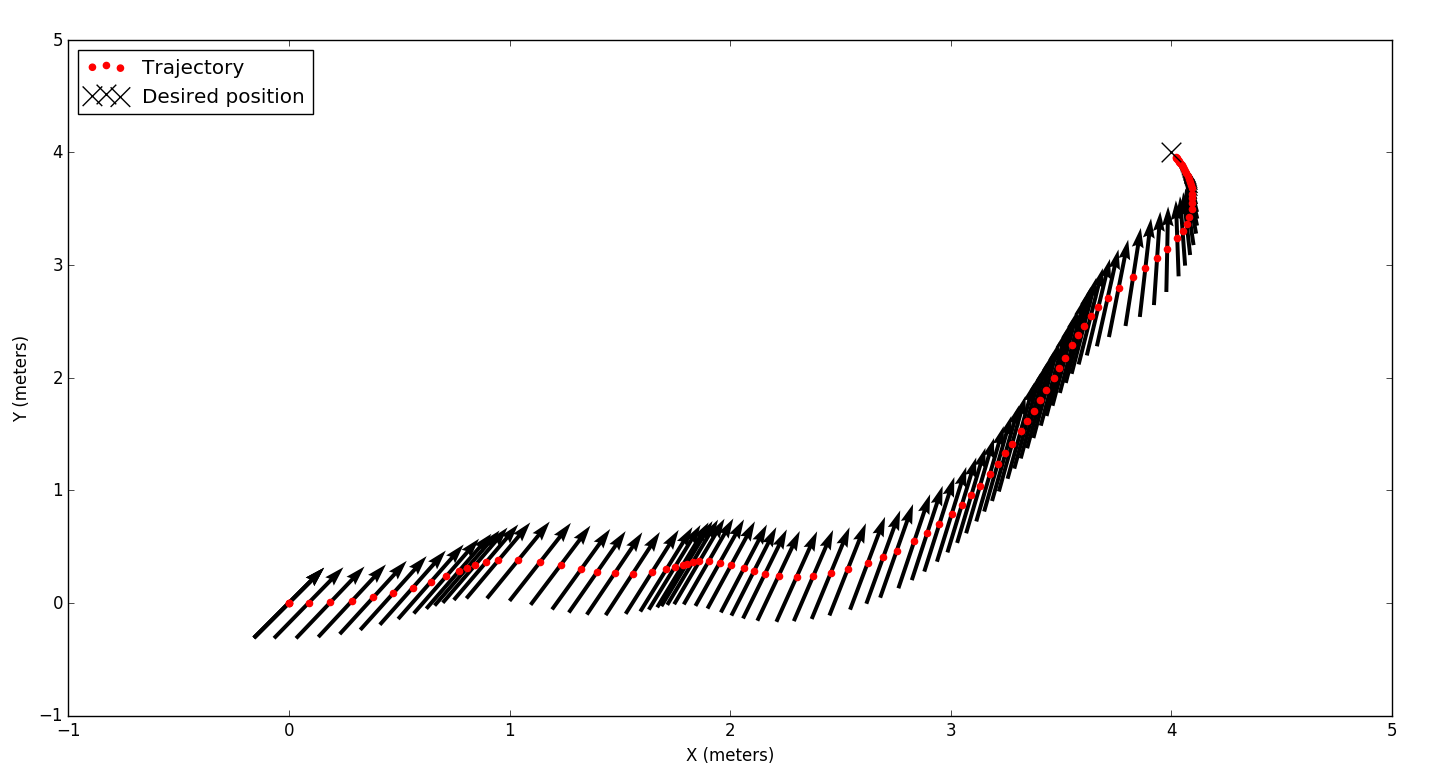
\includegraphics[width = 70mm]{attr_kbki.png}}\\
	\subfloat[Repulsive force applied to the mobile robot] {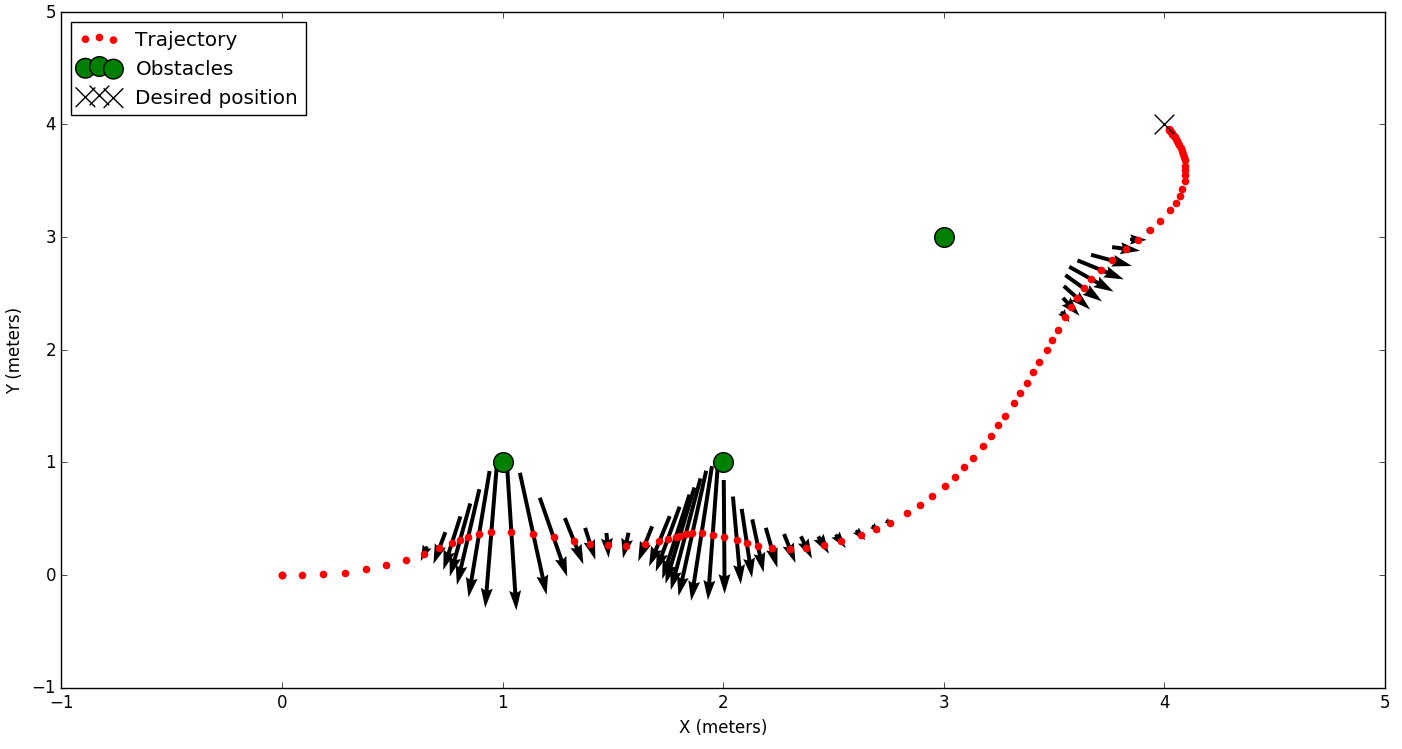
\includegraphics[width = 70mm]{rep_kbki.png}}\\
	\subfloat[Navigation force applied to the mobile robot]{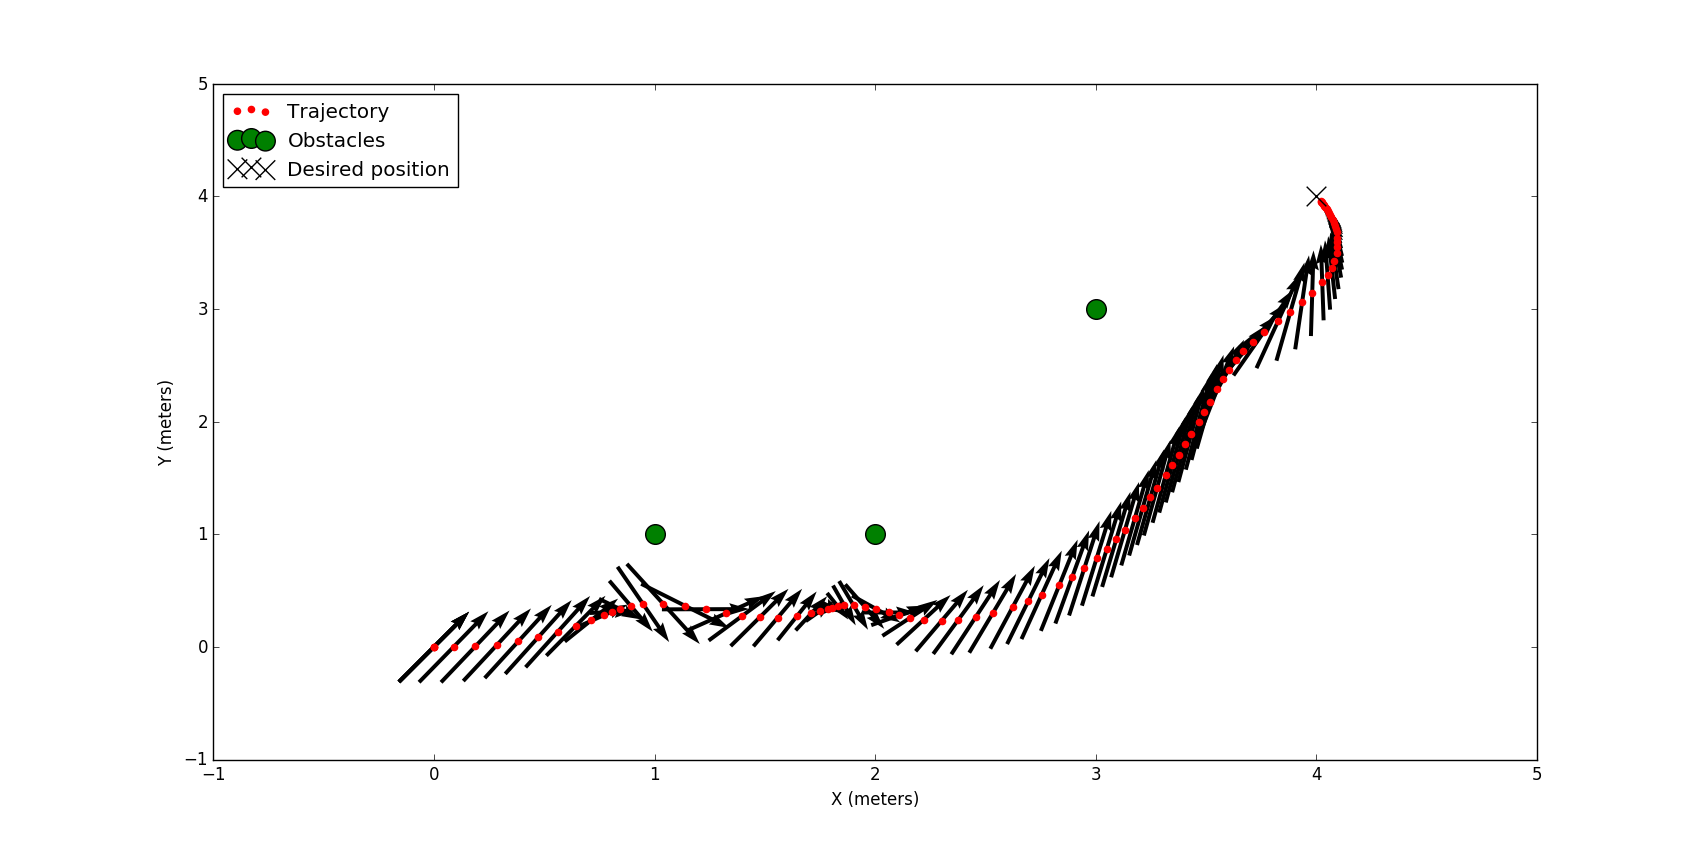
\includegraphics[width = 70mm]{nav_kbki.png}}
	\caption{APF + Polar controller implemented on Kobuki} \label{f:kbki}
\end{figure}

\subsection{Navigation with Lidar}

\begin{figure}
	\centering
	\subfloat[Attractive force applied kobuki with lidar]{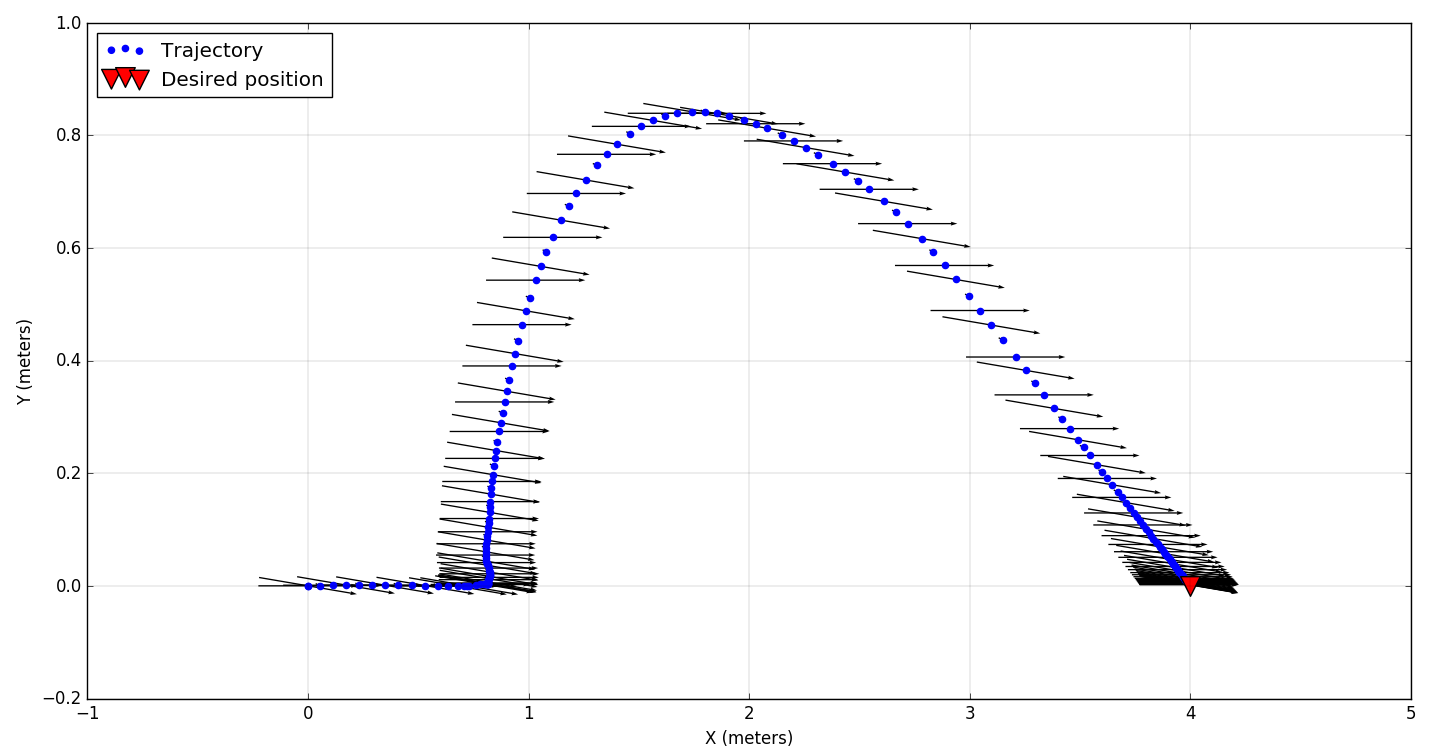
\includegraphics[width = 70mm]{fattr_lidar.png}}\\
	\subfloat[Attractive force applied kobuki with lidar]{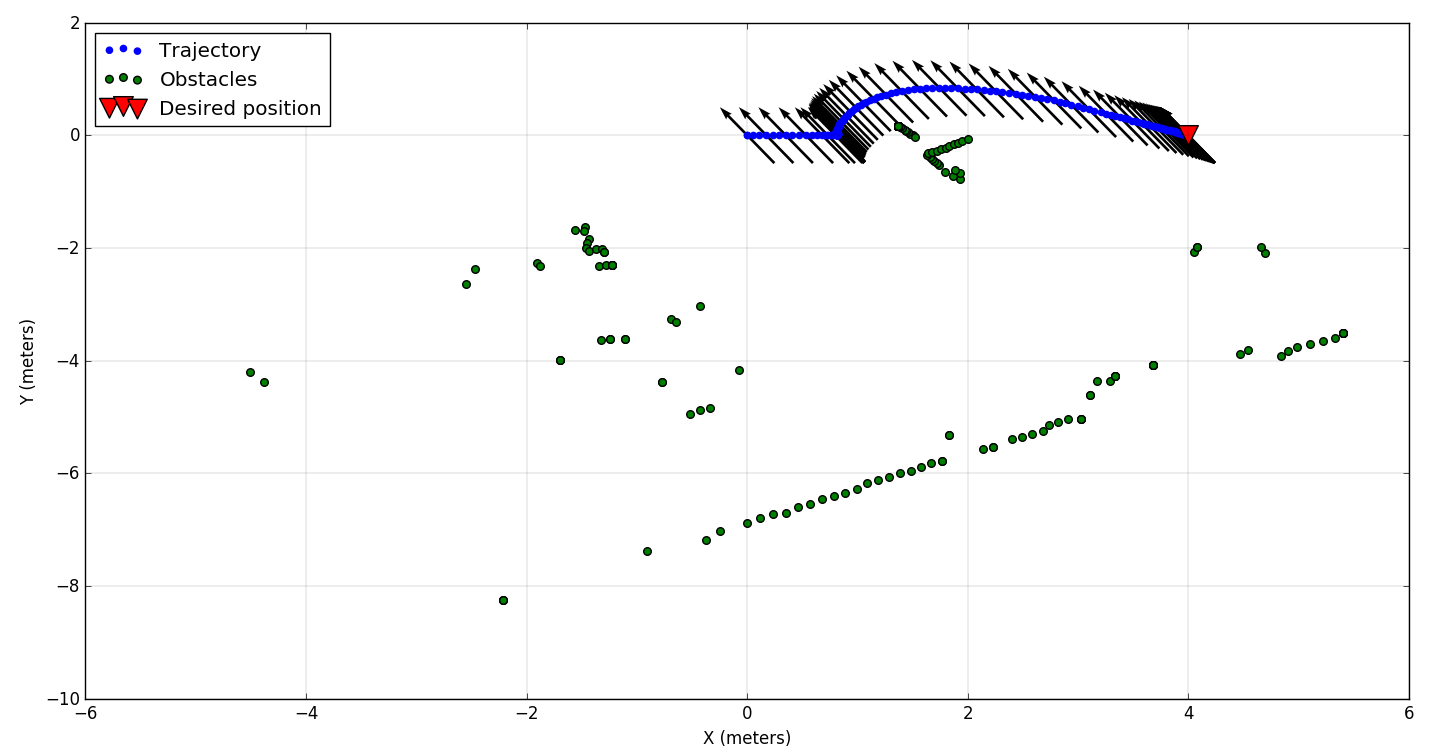
\includegraphics[width = 70mm]{frep_lidar.png}}\\
	\subfloat[Attractive force applied kobuki with lidar]{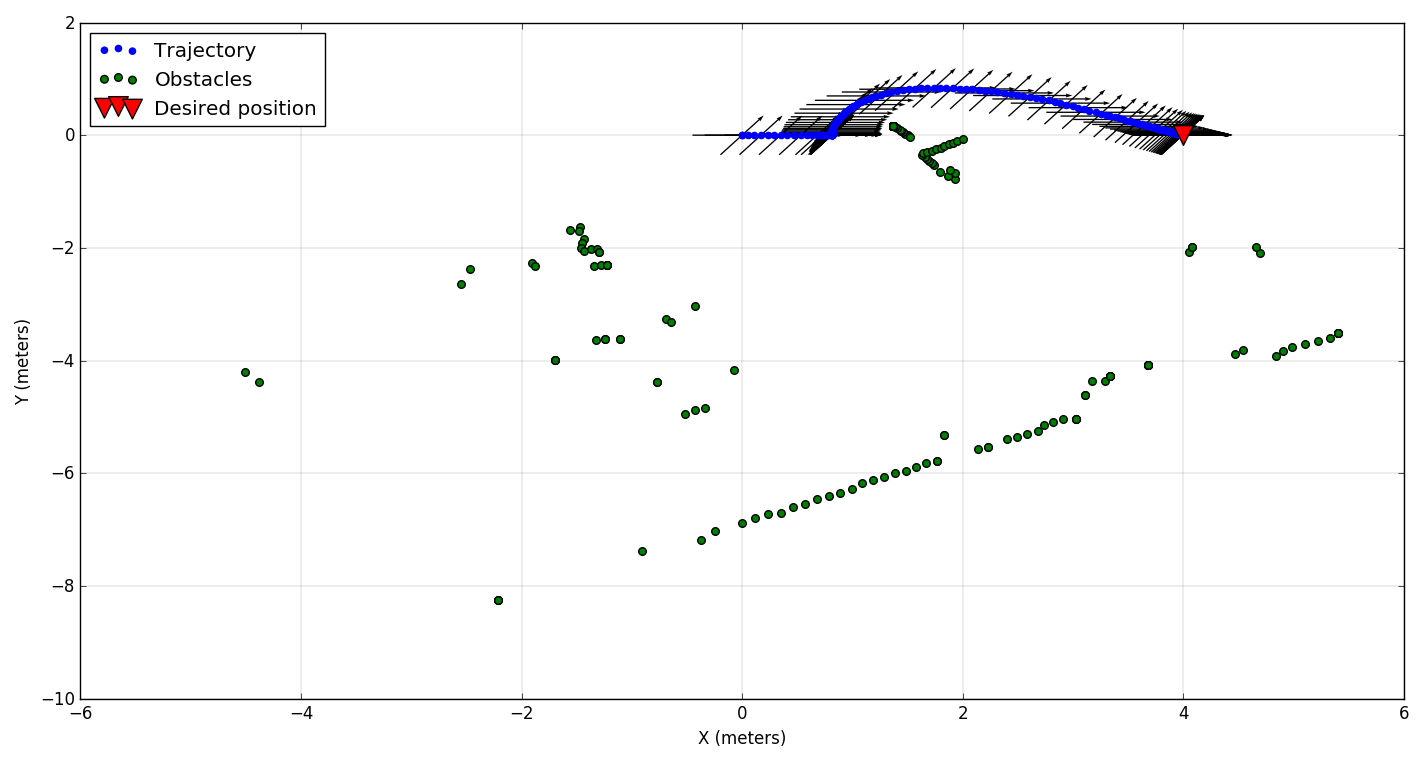
\includegraphics[width = 70mm]{fnav_lidar.png}}\\
\end{figure}

\section{Conclusion}
\label{sec:conclusion}
This paper presented a methodology based on obtaining a sequence of points from a given image, and a inverse kinematics controller for the arm of a robot. Image processing based on edge detection, morphological operations and topological skeletonization was able to render an image from which points could be obtained. A numerical approach for inverse kinematics showed a real-time behavior without several delays. The motion of the NAO robot presents some inherent low-level control problems that deviate from the expected results. Future work will address these problems with a more robust control scheme and a cleaner image processing methodology. Also, writing with both hands at the same time will be explored as a capability that a robot can do but a typical human cannot.

\bibliographystyle{IEEEtran}
\bibliography{biblio.bib}
\end{document}

% Prueba